
\begin{figure}[t]
  \centering
  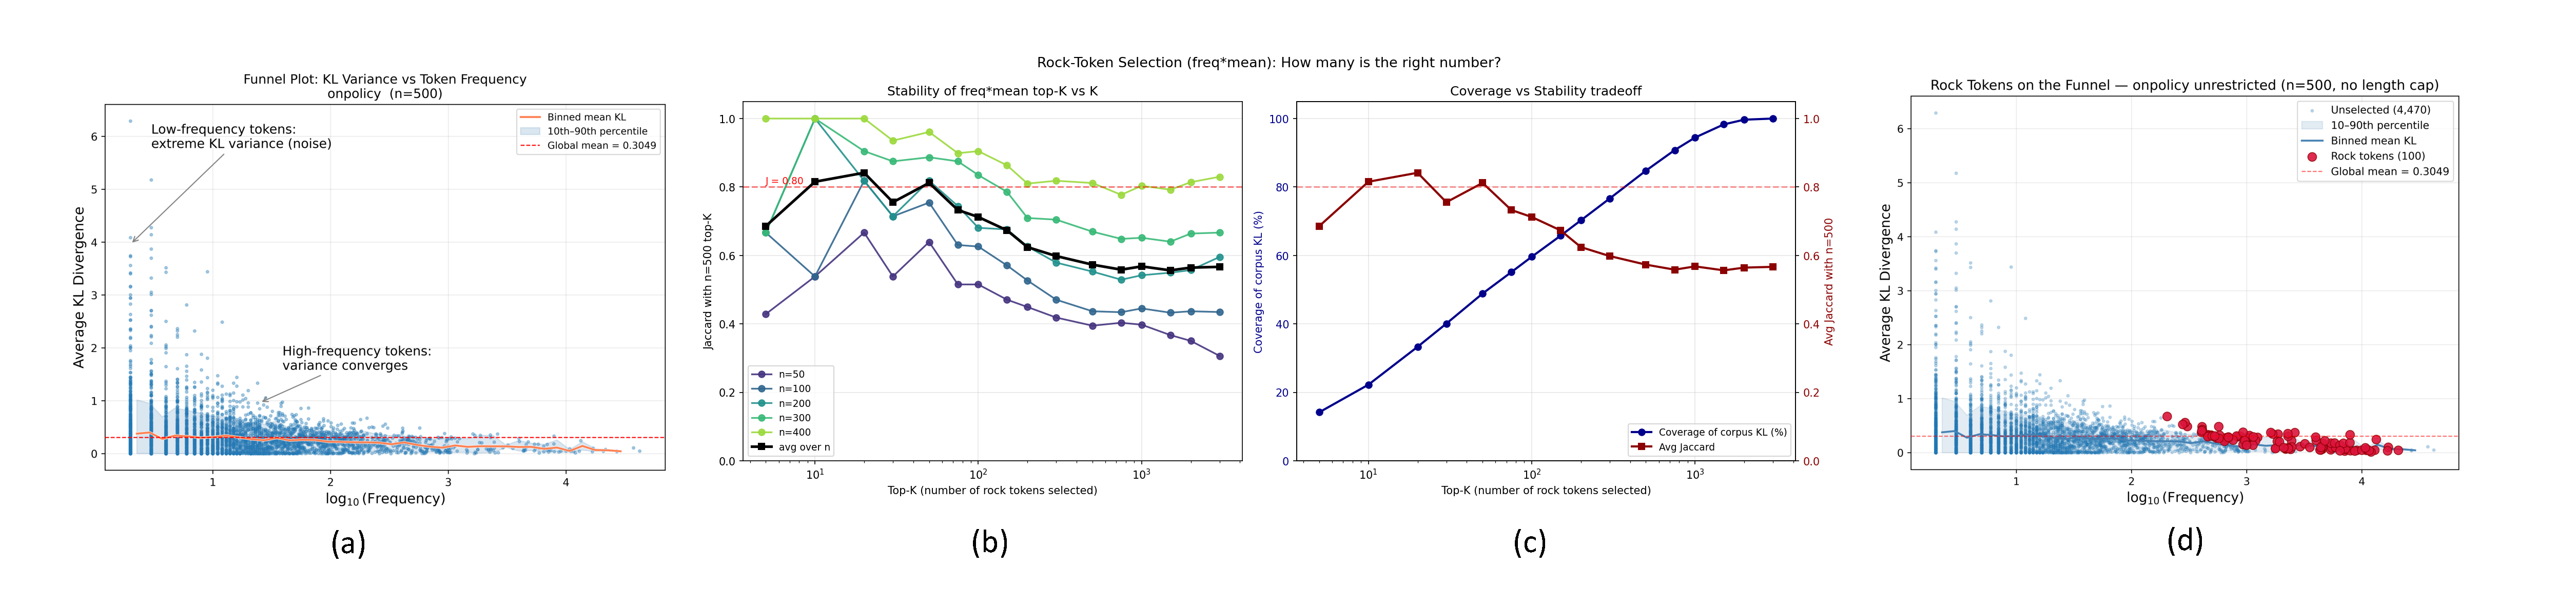
\includegraphics[width=\linewidth]{Figures/Section4/rocktoken.pdf}
  \caption{\textbf{Identification and selection of rock tokens on MATH-500.}
  \textbf{(a)} Per-token reverse KL between OPD-distilled student and teacher,
  plotted against $\log_{10}\mathrm{Freq}(v)$ for every observed token type
  ($n{=}500$). Variance of the per-token mean collapses with frequency: rare
  tokens exhibit extreme but unreliable estimates, whereas high-frequency
  tokens converge toward a corpus-level baseline. Naively ranking by per-token
  mean is therefore dominated by long-tail noise.
  \textbf{(b)} Stability of the top-$K$ set under the proposed score
  $R(v) = \mathrm{Freq}(v) \cdot \mathbb{E}[\ell_t \mid x_t {=} v]$, measured as
  the Jaccard index against the $n{=}500$ reference set when $\widehat R(v)$ is
  estimated from sub-corpora of size $n \in \{50,100,200,300,400\}$ and
  averaged over $n$ (black). The selection remains stable
  ($\bar J \geq 0.70$) for $K \leq 100$ and decays toward a noise floor of
  ${\approx}0.57$ for $K \geq 150$.
  \textbf{(c)} Cumulative coverage of corpus-level KL by the top-$K$ set
  (blue, left axis) and average Jaccard (red, right axis) as functions of
  $K$. The chosen cutoff $K{=}100$ ($\approx 2.5\%$ of the observed
  vocabulary) sits in the stable regime while accounting for ${\sim}60\%$ of
  the total student--teacher KL on the corpus.
  \textbf{(d)} The selected rock-token set $\mathcal{R}$ ($|\mathcal{R}|{=}100$,
  red) overlaid on the funnel. Selected tokens lie at the upper edge of the
  loss distribution within their frequency band and cluster in the mid-to-high
  frequency regime, consistent with $R(v)$'s explicit weighting by evidence.}
  \label{fig:rock-id}
\end{figure}


\subsection{Empirical Analysis}
Recall from §\ref{Preliminaries:Rock Tokens} that rock tokens are token types whose expected per-step KL between student $\pi_\theta$ and teacher $\pi_T$ remains high after on-policy distillation. To identify them empirically, we estimate the per-token loss $\widehat\ell_v = \widehat{\mathbb{E}}\big[D_{\mathrm{KL}}!\big(\pi_\theta(\cdot \mid x_{<t});|;\pi_T(\cdot \mid x_{<t})\big) \mid x_t = v\big]$ from rollouts of the distilled student.

\textbf{Setup} The teacher is Qwen3-30B-Instruct; the student is Qwen3-4B, on-policy distilled on the OpenThoughts dataset. Per-token KL is measured on $N{=}500$ MATH-500 problems, chosen because the dataset elicits the model's reasoning capabilities and yields long, structurally diverse trajectories.

\textbf{Empirical Observations} Figure~\ref{fig:rock-id}(a) plots $\widehat\ell_v$ against $\log_{10}\mathrm{Freq}(v)$ for every observed token type. Two patterns emerge. First, $\mathrm{Freq}(v)$ spans nearly five orders of magnitude — a Zipfian long tail typical of natural-language token distributions. Second, the tokens with the most extreme $\widehat\ell_v$ are concentrated at the lowest frequencies, where each estimate is computed from only a handful of occurrences.

\textbf{The Challenge} The two observations together imply a statistical reliability problem: an extreme $\widehat\ell_v$ at low frequency is indistinguishable from a small-sample artifact of a token that, at higher frequency, would regress toward a moderate mean. Naively ranking tokens by $\widehat\ell_v$ therefore conflates genuinely recalcitrant tokens with rare-event noise. 

\subsection{Proposed Detection Method}

To solve the problem, we consider aligning with the OPD objective and propose detection score $R(v)$. Since $\mathcal{L}{\text{OPD}}$ is an expectation over student trajectories, it admits an exact additive decomposition over token types:
\begin{equation}
\mathcal{L}{\text{OPD}}(\theta)
;=;
\mathbb{E}{x \sim \pi\theta} \sum_{t} \ell_t
;=;
\sum_{v}
\underbrace{\mathrm{Freq}(v) \cdot \mathbb{E}[\ell_t \mid x_t = v]}_{R(v)}.
\end{equation}
The rock score $R(v)$ defined in §\ref{Preliminaries:Rock Tokens} is therefore the exact contribution of token type $v$ to the loss that OPD minimizes. Ranking tokens by $R(v)$ is the unique additive ranking that agrees with the OPD objective.

This form also resolves the statistical reliability problem identified in §X.1. The $\mathrm{Freq}(v)$ factor up-weights tokens whose mean-loss estimate $\widehat{\mathbb{E}}[\ell_t \mid x_t = v]$ converges quickly under sampling, and down-weights rare tokens whose mean is dominated by small-sample noise. Detection by $R(v)$ thus simultaneously aligns with the theoretical objective and is robust to the long-tailed estimation noise in §X.1.

Operationally, $R(v)$ favors tokens with substantial occurrence count and above-baseline per-token loss; rare tokens with extreme observed loss receive low scores because the $\mathrm{Freq}(v)$ weight is small. Section §X.3 confirms this empirically, showing that the top-ranked tokens lie in the mid-to-high frequency range and at the upper edge of the loss distribution within their frequency band, while rare-but-extreme tokens — whose unreliability §X.1 highlighted — fall well outside the selection.


\subsection{Selection of Ratio}
Choosing the selection size. The score $R(v)$ provides a ranking; we still need a cutoff $K$ that determines $|\mathcal{R}|$. Two competing criteria bear on this choice. First, $K$ should be small enough that the top-$K$ set is stable — i.e., reproducible across resamplings of the rollout corpus. Second, $K$ should be large enough that $\mathcal{R}$ accounts for a substantial fraction of the corpus-level KL, so that reweighting decisions made on $\mathcal{R}$ have meaningful effect on $\mathcal{L}_{\text{OPD}}$.

\textbf{Procedure} We sweep $K$ jointly with sample size. For each $n \in {50, 100, 200, 300, 400}$, we compute $\widehat R(v)$ from the corresponding sub-corpus and select its top-$K$ tokens; we then measure the Jaccard index of this set against the top-$K$ obtained at $n = 500$. We additionally compute the cumulative coverage $\sum_{v \in \mathcal{R}} \widehat R(v) / \mathcal{L}_{\text{OPD}}^{\text{corpus}}$ at $n = 500$ as $K$ grows.

\textbf{Results} Figure~\ref{fig:rock-id}(b) plots Jaccard against $K$, with one curve per $n$ and an averaged curve. Average Jaccard exceeds $0.70$ for $K \leq 100$ and decays toward a $\approx 0.57$ floor for $K \geq 150$ — beyond which the additional tokens are no longer reliably reproduced across sub-corpora. Figure~\ref{fig:rock-id}(c) overlays the corresponding coverage curve: at $K = 100$, $\mathcal{R}$ accounts for $\approx 60\%$ of the corpus-level KL while remaining within the stable regime. We therefore set $K = 100$ ($\approx 2.5\%$ of the observed vocabulary) for the remainder of the paper. This choice represents an explicit tradeoff: $K = 50$ would yield modestly higher stability ($J \approx 0.81$) but reduce coverage to $\approx 49\%$.

\subsection{Analysis on Rock Tokens}
 We decode the top-$K{=}100$ rock tokens and their frequency-matched controls $\mathcal{S}_{\text{ctrl}}$ from §\ref{Preliminaries:Frequency-Matched Control} into their string forms using the public Qwen3 tokenizer. Despite being identified by a purely numerical criterion ($R(v)$), the resulting set is functionally coherent: rock tokens fall into a small number of identifiable categories, all of which mark structural or discourse boundaries in mathematical reasoning output.

Four functional clusters dominate $\mathcal{R}$.
\begin{enumerate}
\item \textbf{LaTeX and math delimiters} — \$', \verb|\\|, \verb|$$|, \verb|=|, \verb|^|, \verb|{|, \verb|}|, \verb|frac|, \verb|(|, \verb|)|. These mark transitions into and out of math mode and operate at the syntactic boundary between prose and formula.   \item \textbf{Markdown and whitespace structure} — **', \textbackslash n', \textbackslash n\textbackslash n', :\textbackslash n\textbackslash n', ---\textbackslash n\textbackslash n', \#\#\#'. These delimit logical units (paragraphs, section headers, bold spans).   \item \textbf{Discourse markers at sentence-initial position} — So', Let', We', But', Now', Wait', Then', Since', This'. These open new reasoning steps and signal turns in the chain of thought.
\item \textbf{Digits} — every digit 0' through 9' appears in $\mathcal{R}$, each with frequency in the thousands and a non-trivial mean per-token KL. These are tokens that punctuate quantitative statements.
\end{enumerate}

Contrast with the frequency-matched control set. The control set $\mathcal{S}_{\text{ctrl}}$, sampled at the same frequency distribution, is qualitatively different: it consists predominantly of content-bearing tokens used at non-boundary positions — common nouns and verbs of mathematical discourse (e.g.\ triangle', equation', region', expression', must', find', check'), prepositions and conjunctions used mid-clause (as', between', first', right'), and single-letter variable tokens (a', b', i', f', y'). The frequency-matching procedure thus isolates the relevant axis: rocks and controls share the quantity of supervision they receive during OPD, but differ sharply in their syntactic role.

\textbf{Interpretation} The clustering of $\mathcal{R}$ at structural boundaries indicates that the residual student–teacher divergence after on-policy distillation is concentrated at the points where the model decides \emph{how to structure} its reasoning output, rather than \emph{what content} to emit. Decisions like open math mode'', begin a new paragraph'', insert a section header'', or start a new reasoning step with So' versus Then','' are precisely the positions where the OPD loss persists, even after extensive distillation. This observation suggests that rock tokens are not arbitrary statistical outliers but a consistent signature of the on-policy distillation regime: they identify the structural/discourse decisions that the student systematically fails to align with the teacher.